\section{Newsfeed App - Recherchebericht}
\label{section:realisation:newsfeed_app}


Newsfeed App for deskless/frontline employees Firstline workers
\begin{itemize}
\item {Mircosoft Staffhub https://products.office.com/de-de/microsoft-staffhub/staff-scheduling-software}
\item {Inkling 	https://www.inkling.com/ }
\item {Zinc https://www.zinc.it/ Beliebteste/Am häufigsten genutzte App für „Deskless“ Mitarbeiter}
\item {Slack https://slack.com/intl/de-de Desktop worker or/and Frontline worker?}
\item {Nicht geeignet: Whatsapp Business https://www.deutsche-handwerks-zeitung.de/whatsapp-betrieblich-nutzen-was-beim-datenschutz-wirklich-gilt/150/3101/363865}
\end{itemize}


\subsection{Lastenheft}
\begin{itemize}
\item Es ist ein Recherchebericht zu erstellen, der sich mit Produkten, Lösungen und Anwendungen (im Folgenden als Anwendungen zusammengefasst) befasst. Konkret geht es um Anwendungen, die es Unternehmen ermöglichen, ihre Mitarbeiter über unternehmensinterne Vorgänge zu informieren und den Mitarbeitern eine Interaktion mit dem Unternehmen ermöglichen. 
\item Der Bericht soll eine Übersicht über die am Markt etablierten Anwendungen liefern. Ein Fokus soll auf den Anreizen liegen, mit welchen die Anwendungen die Mitarbeiter zur Benutzung motivieren.
\item Des Weiteren soll im Bericht untersucht werden, welche Umfragefunktionalitäten in der jeweiligen Anwendung bereits existieren und wie diese potentiell durch PulseShift genutzt werden könnten. 
\item Darüber hinaus soll der Bericht aufzeigen, welche weiteren Möglichkeiten zur Einbindung einer Umfrage durch PulseShift es jeweils gibt und wie flexibel diese Möglichkeiten genutzt werden können.
\item Außerdem sollen in dem Bericht die Erfahrungen von Referenzkunden, die die Anwendung bei Offline-Mitarbeitern einsetzen, beschrieben werden. 
\item Sofern jeweils eine Preisstruktur verfügbar ist, soll außerdem auf diese eingegangen werden.
\end{itemize}

\subsection{Pflichtenheft}
\begin{itemize}
\item Es wird ein Recherchebericht erstellt, der sich mit Produkten, Lösungen und Anwendungen (im Folgenden als Anwendungen zusammengefasst) befasst. Konkret wird es um Anwendungen gehen, die es Unternehmen ermöglichen, ihre Mitarbeiter über unternehmensinterne Vorgänge zu informieren und den Mitarbeitern eine Interaktion mit dem Unternehmen ermöglichen.
\item Der Bericht wird eine Übersicht über die am Markt etablierten Anwendungen liefern. Für die Marktführer wird herausgearbeitet, mit welchen Anreizen sie die Mitarbeiter zur Benutzung der Anwendung motivieren. Sofern jeweils möglich werden die Anwendungen dazu neben einer Internetrecherche auch aktiv getestet.
\item Des Weiteren werden im Bericht die Möglichkeiten zur Integration der Umfrage von PulseShift in die jeweilige Anwendung aufgezeigt. Diese wird tabellarisch mit zusätzlichen erläuternden Texten gegenübergestellt. Dabei wird sofern jeweils verfügbar sowohl auf die Umfragefunktionalitäten der Anwendung als auch das Abspringen zur Umfragefunktion von PulseShift eingegangen. Außerdem werden jeweils mögliche weitere anwendungsspezifische Möglichkeiten wie beispielsweise ein Einbinden der Umfrage mittels iFrame vorgestellt.
\item Abschließend werden die Erfahrungen von Referenzkunden dargelegt. Dabei wird der Fokus auf Erfahrungen liegen, die im unmittelbaren Zusammenhang mit dem Einsatz bei Offline-Mitarbeitern stehen.
\item Der Bericht wird innerhalb des Projektabschlussberichts in Latex erstellt.
\end{itemize}


\subsection{Firstline Worker}

Die Firstline Workforce klassifiziert alle Mitarbeiter ohne festen Computer-Arbeitsplatz. Sie repräsentieren die mehr als zwei Milliarden Menschen  in Rollen, die sie zum ersten Kontaktpunkt zwischen einem Unternehmen und der Außenwelt machen. Sie sind die Menschen hinter der Theke, am Telefon, in den Kliniken und in der Werkstatt. Sie bilden das Rückgrat vieler der weltweit größten Branchen - Einzelhandel, Restaurants, Gastgewerbe, Reisen, Fertigung und Bauwesen. In dieser Rolle sind sie oft die ersten, die Kunden ansprechen, die ersten, die die Marke eines Unternehmens repräsentieren und die ersten, die Produkte und Dienstleistungen in Aktion sehen.


\begin{figure}[H] 
\centering 
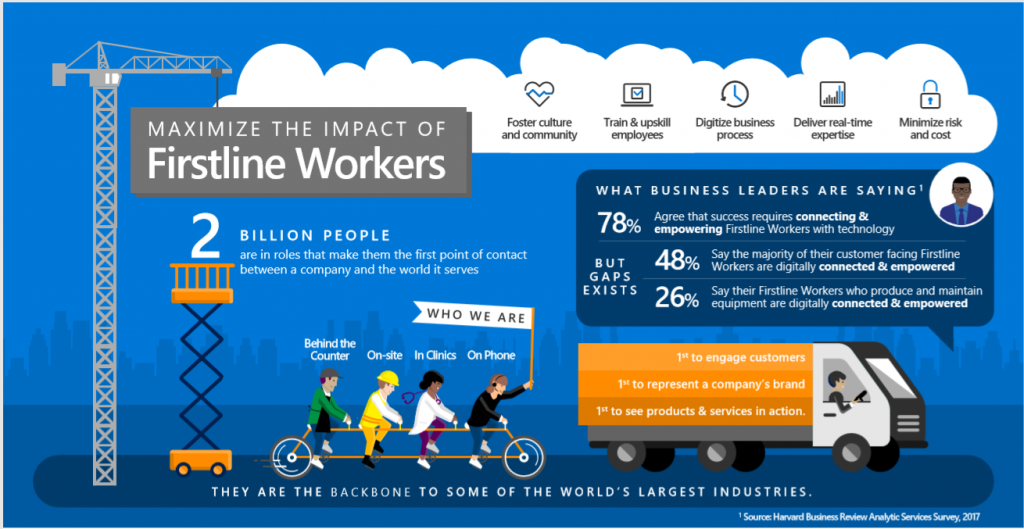
\includegraphics[scale=0.48]{images/frontlineworkers} 
\caption[Frontline Workers]{Frontline workers\protect} 
\label{dem} 
\end{figure}


\subsection{Microsoft Staffhub}





\subsection{Cotap}
Cotap ist eine von Zinc entwickelte mobile Nachrichtenapplikation für das Unternehmensumfeld. Sie ist insbesondere für \glqq Deskless\grqq Unternehmen geeignet. Es soll dem Unternehmen ermöglichen schnell und einfach mit seinen Mitarbeitern zu kommunizieren. 

Die Funktionalitäten der Applikation lassen sich in zwei Hauptkategorien aufteilen. 

\begin{itemize}
\item Kommunikationstools - zur Kommunikation im Unternehmen 
\item Analysetools - zur Analyse des Kommunikationsverhalten und somit auch zur Analyse der Unternehmenssituation
\end{itemize}

Folgend werden diese Tools aufgegliedert in die einzelnen Funktionsbereiche vorgestellt.

\subsubsection{Kommunikationstools}

\begin{itemize}
\item 1:1 Messages - senden von direkten Nachrichten an jedem aus der Organisation
\item Group Messages - um sich beispielsweise innerhalb einer Abteilung abzustimmen
\item Content Sharing - um Dokumente und weitere wichtige Informationen mit anderen Mitarbeiten zu teilen
\item Hands Free - Nachrichten werden laut vorgelesen und können eingesprochen werden
\item 3RD Party Messaging - Personen, die nicht der eigenen Organisation zugeordnet sind können einfach über die E-Mail-Adresse hinzugefügt werden
\item Push to Talk - Schnelle und einfache Benachrichtigung anderer Mitarbeiter oder Gruppen durch Walkie Taklie Funktion
\item Broadcast - zum Versenden dringender und wichtiger Nachrichten an alle Beteiligten, zusätzliche Funktionalität eines Pop-Ups
\end{itemize}

Die drei letzte Komponenten 3RD Party Messaging, Push to Talk und Broadcast können für unseren Use Case genutzt werden.

3RD Party Messaging kann es PulseShift ermöglichen, über einen Gruppenchat, in welchen sie eingeladen wurden, einen Link zur Umfrage zu posten. So könnten jeweils einzelne Abteilungen gezielt erreicht werden.

Durch Push to Talk kann darauf aufmerksam gemacht werden, dass es eine Umfrage gibt an der man teilnehmen kann. Hier ist es jedoch entscheidend, dass die Übertragung der Nachricht in Tonform und live ist. 

Mit Hilfe des Broadcasts könnte ein Link zur Umfrage versendet werden. So wird dem Mitarbeiter zusätzlich suggeriert, dass es wichtig ist an dieser Umfrage teilzunehmen. 

\subsubsection{Analysetools}
Mit Hilfe der Analysetools werden die gesendeten Nachrichten, hinsichtlich Menge, Inhalt, Länge und weiteren Kriterien analysiert, um weitere Informationen zu generieren. 

Die verschiedenen Analysen werden folgend kurz dargestellt: 

\begin{itemize}
\item Analyse der einzelnen Kommunikationskanäle
\item Historischer Verlauf der Broadcasts
\item Analyse der Anzahl und Größe von gesendeten Nachrichten
\item Networkmap, um zu zeigen wer mit wem kommuniziert
\end{itemize}

Aus diesen Informationen könnte ein Mehrwert für die Umfragen geschlossen werden, dazu wäre jedoch eine komplette Erweiterung des Umfragekonzeptes notwendig und wird daher vorerst verworfen.

\subsubsection{Integrationsmöglichkeiten}
Cotap bietet die Möglichkeit andere Apps zu integrieren, sodass der Nutzer die App nicht verlassen muss, um mit anderen Apps zu interagieren. Mit Hilfe dieser Funktionalität könnten die Umfragen von PulseShift sehr einfach eingebunden werden. 

Außerdem können automatische Benachrichtigungen erstellt werden, um die Mitarbeiter auf die Umfrage hinzuweisen.

\subsubsection{Kosten}
Die App Cotap kann zunächst einmal kostenlos im Playstore herunter geladen werden. Mit Hilfe dieser kostenlosen Version können unbegrenzt Nachrichten gesendet werden, sowie Fotos, Videos und der eigene Standort geteilt werden. Außerdem sind Basic-Integrationen möglich. 

Für 5 Dollar monatlich soll es möglich sein, Audio und Video Anrufe bis zu 100 Minuten pro Nutzer pro Monat zu tätigen und Daten bis zu zwei GB pro User pro Monat zu versenden. In diesem Paket ist außerdem die Gruppenorganisation und Nutzung enthalten. Des weiteren können individuelle Benachrichtigungen erstellt werden.

Das teuerste Paket ist für 10 Dollar pro Monat zu erhalten. Hier können Audio und Video Anrufe bis zu 250 Minuten pro Nutzer pro Monat getätigt werden. Außerdem können unlimitiert Daten versendet und empfangen werden. Nun können Enterprise-files sowie ein Single Sign-One integriert werden. Außerdem wird alles aktiv überwacht und die Analysetools somit genutzt werden.

\subsubsection{Bewertung}
Cotap erscheint als eine gute Möglichkeit, um die Umfragen von PulseShift zu integrieren. Die genaue Zusammenarbeit mit Cotap, PulseShift und dem jeweiligen Unternehmen muss jedoch abgeklärt werden, sowie die genauen Kosten ermittelt werden.
